\documentclass[a4paper]{exam}

\usepackage{graphicx}
\usepackage{siunitx}
\DeclareSIUnit{\revolution}{rev}
\DeclareSIUnit{\rpm}{\revolution\per\minute}
\DeclareSIUnit{\lightyear}{ly}

\begin{document}
  \section*{L3 Physics: Questions for 1.3 (Mechanics, oscillation)}
  The first two questions are past exam questions, from 2013 and 2018 respectively. Remainder from Knight, chapter 15 and Bendall, chapter 10.
  \begin{questions}
    \question A ball, attached to a cord of length \SI{1.20}{\metre}, is set in motion so that it is swinging backwards and forwards like a pendulum.
      \begin{parts}
        \part Show that the period of a pendulum of length \SI{1.20}{\metre} that is oscillating in
              simple harmonic motion is \SI{2.20}{\second}.
        \part Explain what must be done to ensure that the motion of the ball approximates simple harmonic motion.
        \part Sketch a graph to show what happens to the ball's \textbf{total} energy over time until it stops swinging.
        \part It is possible to get the ball swinging by holding the top end of the cord and gently shaking it backwards and forwards.

              Explain how shaking the top end of the cord can make the ball on the bottom of the cord oscillate in simple harmonic motion.

              In your answer, you should consider resonance and energy transfer.
        \part Simple harmonic motion requires a restoring force that changes in proportion to the size of the displacement.

              Discuss what provides the restoring force when the ball is swinging in simple harmonic motion.

              In your answer, you should:
          \begin{itemize}
            \item describe what forces act on the ball
            \item explain how these forces change as the ball swings
            \item draw vectors to show how a restoring force is produced
          \end{itemize}
      \end{parts}
    \question A railway wagon full of sand is released from rest at point C. The wagon oscillates on a vertically
              curved track between A and C with simple harmonic motion of period \SI{60.0}{\second}. The effects of friction
              can be ignored.

              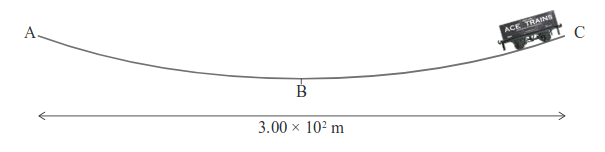
\includegraphics[width=0.8\textwidth]{shmtrain-nzqa2018}
      \begin{parts}
        \part
          \begin{subparts}
            \subpart State the conditions that must apply for the motion to be simple harmonic motion.
            \subpart Show that the maximum speed attained is \SI{15.7}{\metre\per\second}.
          \end{subparts}
        \part When the wagon is halfway between B and C, calculate its approximate height above B.
        \part
          \begin{subparts}
            \subpart
              The wagon has a small hole from which sand leaks onto the flat ground beneath the rail track at a steady rate.
              Sketch a height profile of the sand on the graph below and explain the shape of the
              profile. State any assumptions made.

              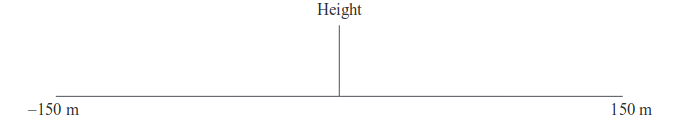
\includegraphics[width=0.8\textwidth]{shmsand-nzqa2018}
            \subpart
              When the wagon arrives back at C, the remaining sand is suddenly dumped from the wagon.
              Explain what effect this removal of mass will have on the physical parameters of the wagon’s motion.
          \end{subparts}
        \part The track A to C is an arc of a circle.

              By first calculating the radius of the circle, discuss whether the original assumption that this
              motion is simple harmonic motion is valid.
      \end{parts}
    \question Suppose a large spherical object (e.g. a planet), of mass $ M $ and radius $ R $, has a narrow tunnel
              passing diametrically through it. A particle of mass $ m $ is inside the tunnel at a distance $ x \leq R $
              frokm the centre. It can be shown that the net force on the particle is due entirely to the sphere of mass with
              radius $ x $; there is no net gravitational force from the spherical shell outside this sphere.
      \begin{parts}
        \part Find an expression for the gravitational force on the particle, assuming the large object has uniform density.
              Your expression should be in terms of $ x $, $ m $, $ M $, $ R $, and any necessary constants.
        \part In (a) you should have found that the gravitational force is a net restoring force. Consequently, in the absence
              of air resistance, objects in the tunnel will oscillate with SHM. Suppose an astronaut exploring a \SI{150}{\kilo\metre}
              diameter, \SI{3.5e18} asteroid discovers a tunnel through the centre. If she jumps into the hole, how long
              will it take her to fall through the asteroid and out the other side?
      \end{parts}
    \question For a particle in simple harmonic motion, show that $ v_\text{max} = (\pi/2) v_{\text{avg}} $ (where $ v_{\text{avg}} $ is
              the average speed during one cycle of the motion).
    \question A grandfather clock ticks each time the pendulum passes the lowest point. Roughly how long must the pendulum be for
              the ticks to occur once a second?
    \question A spring is hung from the ceiling. When a block is attached to its end, it stretches \SI{2.0}{\centi\metre} before
              reaching its new equilibrium point. The block is then pulled slightly down and released. What is the frequency of the
              resulting oscillation?
    \question Sarah bounces on a trampoline. As long as the amplitude of her motion is small, she stays in contact with the mat throughout
              each oscillation and her motion is approximately modelled by SHM. She bounces at a frequency of \SI{1.1}{\hertz}, and an
              initial amplitude of \SI{0.15}{\metre}.
      \begin{parts}
        \part Show that it takes Sarah \SI{0.12}{\second} to drop \SI{0.11}{\metre} below her rest position.
        \part If Sarah is \SI{0.11}{\metre} below her rest position:
          \begin{subparts}
            \subpart Calculate her speed;
            \subpart State and explain the direction of her acceleration; and
            \subpart Calculate the magnitude of her acceleration.
          \end{subparts}
        \part Calculate Sarah's maximum speed, and explain when she will be travelling at this speed.
        \part Calculate Sarah's maximum acceleration, and explain when she will reach this acceleration.
      \end{parts}
    \question The bob of a simple pendulum has mass \SI{0.25}{\kilo\gram} and maximum speed \SI{1.8}{\metre\per\second}.
      \begin{parts}
        \part Calculate the vertical height of the bob above its equilibrium point when it was released.
        \part Explain why, over time, the amplitude of oscillation of the pendulum will decrease.
        \part Discuss the effect of an oscillating driving force on the pendulum.
      \end{parts}
  \end{questions}

\vspace*{\fill}
This version: \today

\end{document}
